\documentclass{article}
\usepackage[utf8]{inputenc}
\usepackage{xeCJK}
\usepackage{bm}
\usepackage{amsmath,amssymb}


\title{ASR Principia 《ASR之道-数学篇(图论)》}
\author{xiao11lam/ZHANG XIAO }
\date{June 2020}

\usepackage{natbib}
\usepackage{graphicx}

\begin{document}

\maketitle
\begin{abstract}
欧拉为解决科尼斯堡七桥问题而有了图论,并提出和解决了“一笔画”的问题。Ps.科尼斯堡曾为普鲁士首府,在二战后划归苏联,现名加里宁格勒是俄罗斯联邦的一部分,却与俄罗斯相隔甚远,可以说是其飞地。而当地主要也以俄语为主要语言。康德,霍夫曼,希尔伯特等都出生在这里。
\end{abstract}

\section{Graph}
\bm{$Graph\ theory $} studies \bm{$graphs$} . one \bm{$graph$} contains several vertices(节点) and edges(边).  It denotes as G = <V, E>. 

\begin{figure}[h!]
\centering
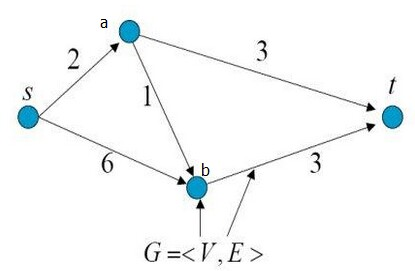
\includegraphics[scale=0.7]{fig1}
\caption{Graph}
\label{fig:ss}
\end{figure}

\begin{flusleft}
Like G = <V, E>,
\quad 
     V = \left\{a, b, S, t\right\},
\quad
     E = \left\{
         \left\{a, b\right\} 
         \left\{a, t\right\} 
         \left\{b, t\right\} 
         \left\{S, a\right\} 
         \left\{S, b\right\}
         \right\}.
\end{flusleft}

\section{Categories of Graph}
\begin{itemize}
    \item  Simple Graph(简单图)
    
    
\begin{flushleft}
\end{flushleft}
    \item  Complete Graph(完全图)
    
\begin{flushleft}
\end{flushleft}
    \item  Isolated Vertex(孤立结点)

\begin{flushleft}
\end{flushleft}
    \item  Null Graph(零图)
\end{itemize}
    
\section{Weighted Graph}
Weighted Graph G = <V, E, f, g>\\
\begin{flushleft}
Vertice Weighted Function: f:V \rightarrow{$W$}
\\
Edge Weighted Function: g:E \rightarrow{$W$}
\\
\quad W can be any set. 
\\
\quad Weighted Graph adds the weights info to common graphs, for letting us to find the "Optimal Path"(最优路径) instead of "Shortest Path"(最短路径).
\end{flushleft}

\section{Degree and Regular Graph}
\begin{flushleft}
The degree of one particular vertice(V) describes the quantity of the edges out or in that V. So d(v) = d+(v) + d-(v).
\end{flushleft}

\begin{flushleft}
d+(v) is the total number of edges starts from that vertice "v".
\end{flushleft}

\begin{flushleft}
d-(v) is the total number of edges ends at that vertice "v".
\end{flushleft}

\begin{flushleft}
If in a graph, all the vertices have the same degree, then we call it \bm{$Regular\ Graph$}.
In this case, we denote the d(v)=k, so we call that graph \bm{K-Regular\ Graph}
\end{flushleft}

\begin{figure}[h!]
\centering
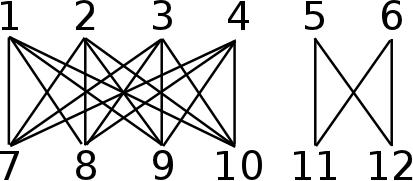
\includegraphics[scale=0.4]{K-regular_graph}
\caption{K-regular_graph}
\label{fig:ss}
\end{figure}
\begin{flushleft}
In Fig2, we can denote into: "K_{4}\ Regular\ Graph" and "K_{2} \ Regular  \ Graph".
\end{flushleft}


\section{Subgraph and Isomorphic}
\begin{flushleft}
G_{1}=<V_{1}, E_{1}>\\
G_{2}=<V_{2}, E_{2}>\\
If V_{1} \subseteq V_{2}, E_{$1$} \subseteq E_{$2$}, then \  we \ say \ G_{1} \ is \ a \ subgraph \ of \ G_{2}.
\end{flushleft}

\begin{flushleft}
when:\\
\mid V_{1} \mid = \mid V_{2} \mid \\
\mid E_{1} \mid = \mid E_{2} \mid \\
Then we say they are isomorphic.
\end{flushleft}

\begin{figure}[h!]
\centering
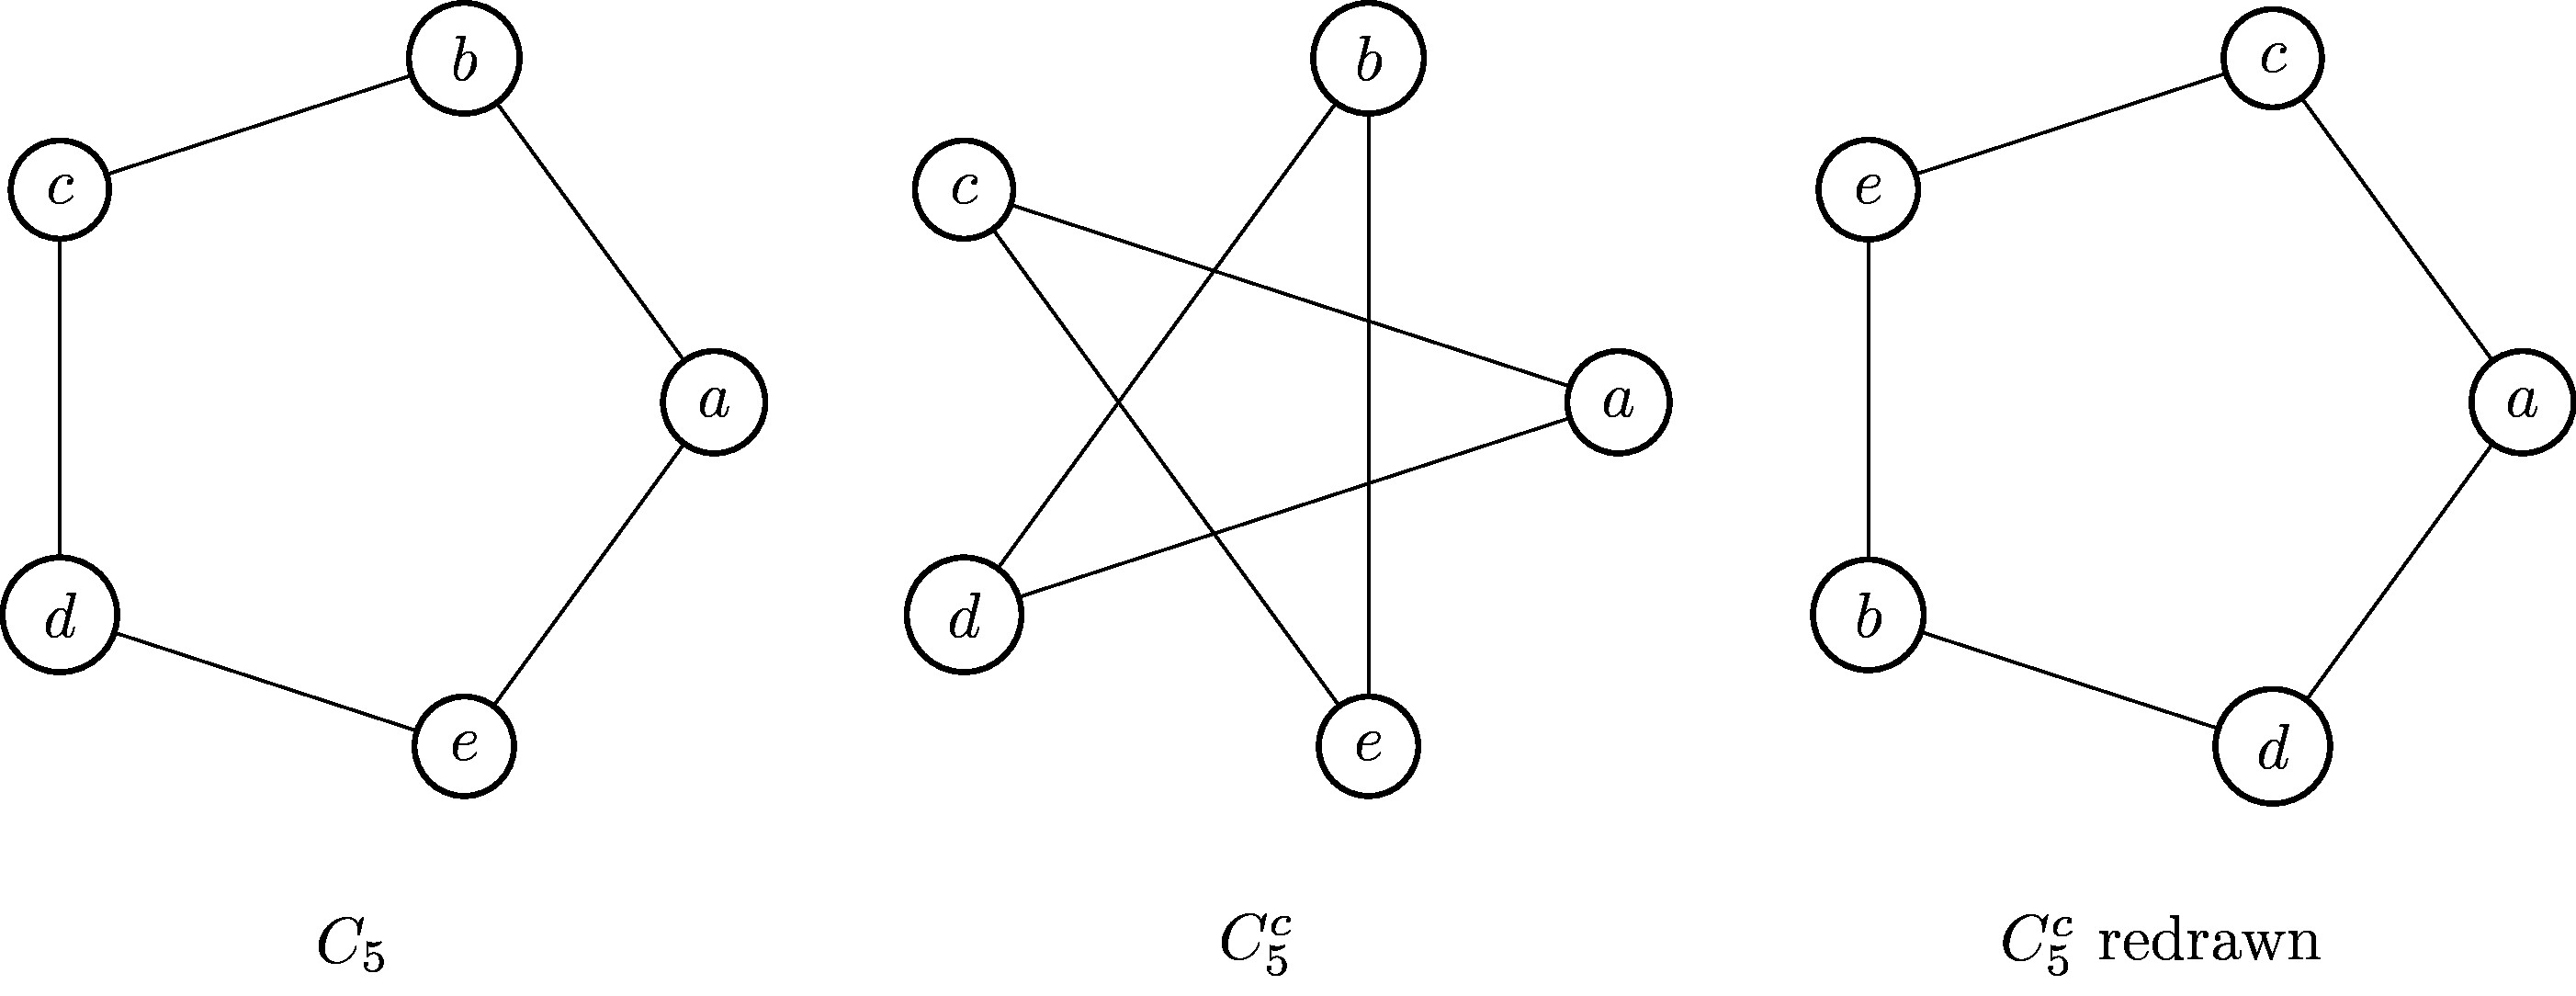
\includegraphics[scale=0.1]{graph_isomorphic}
\caption{Isomorphic}
\label{fig:ss}
\end{figure}

\section{Walk and Path (路径和通路)}
\subsection{Pseudo Path(拟路径)}
\begin{flushleft}
Just like walk from some point to another place, recording the route.
\end{flushleft}

\begin{figure}[h!]
\centering
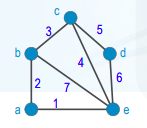
\includegraphics[scale=1]{Pseudo-Path}
\caption{Isomorphic}
\label{fig:ss}
\end{figure}
\begin{flushleft}
From fig4, we can set two paths like this:\\
a,1,e,7,b,3,c,3,b,2,a\\
c,4,e,4,c,3,b,7,e,4,c\\
The length of the path is the number of edges it crossed.
\end{flushleft}

\subsection{Walk and Path}
\begin{flushleft}
If the vertices in Pseudo-path are different, then we call they are "Walk"\\
like: \bm{a,1,e,7,b,3,c,3,b,2,a}\\
If the edges in Pseudo-path are different, then we call they are "Path"\\
like: \bm{c,4,e,4,c,3,b,7,e,4,c}\\
\end{flushleft}

\subsection{Accessibility}
\begin{flushleft}
If U_{$access$}V\\
means that there exists a route can connect from U to V.
\end{flushleft}

\end{document}
